In this chapter, the requirements of a system that can solve the problem described in the problem definition, in chapter \ref{problemdefinition} has been defined. This has been done by first exploring different use cases for the system and then analyzing them to get a formal list of requirements.

\section{System behaviour}
\label{sec:system-behaviour}
To better understand how the system, developed through out this report, could work, this section contains a description of actual situations, that we imagine the system could be used in. This includes descriptions of how each part of the system should respond to an event.

The system should be activated upon one of the following conditions, that triggers during or after the falling accident has happened:

\begin{itemize}
    \item The citizen activates the system manually
    \item The smartphone detects a falling event
    \item The personal assistant detects a falling event
\end{itemize}

When the smartphone detects a falling event, it should wait a short while for user response, either in the form of a button-press or voice-detection. This would allow for the user to interrupt the process, and therefore avoid emergency services or contact person being contacted when they are not needed. When a short while has passed, and no user interaction has happened, it should begin to contact people from that citizen contact list in the priorities order, this process can be seen on graph \ref{fig:SmartPhoneApp}.

\begin{figure}[H]
    \centering
    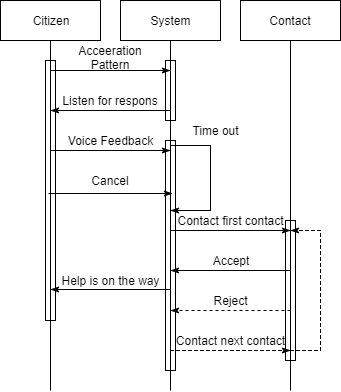
\includegraphics[width=0.5\textwidth]{Figures/Phone.png}
    \caption{Sequence diagram for smartphone app}
    \label{fig:SmartPhoneApp}
\end{figure}

When the personal assistant detects a falling accident it should verify that a falling accident has actually taken place, and then notify the system that the citizen has fallen and activate an alarm in the system. The personal assistant receives confirmation that help has been requested and who has responded to it. The personal assistant should be context aware, so that it doesn't call for help during normal dialogue, and in general try to distinguish between false positives. This process can be seen on graph \ref{fig:PersonAssitent}

\begin{figure}[H]
    \centering
    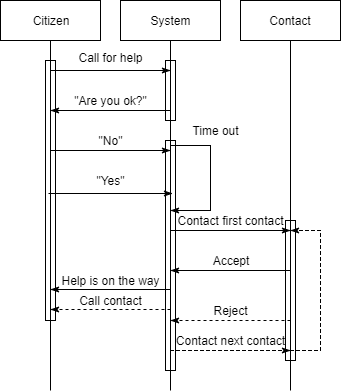
\includegraphics[width=0.5\textwidth]{Figures/PersonAssitent.png}
    \caption{Sequence diagram for personal assistant}
    \label{fig:PersonAssitent}
\end{figure}

When the system gets an alert of a falling event it looks up the citizen in need of help, and find their contact list. It then tries to contact people on the contact list until someone on the list responds to the call for help. There should also be an option to call emergency services, if nobody on the contact list responds, this can be seen in \ref{fig:SmartPhoneApp} and \ref{fig:PersonAssitent} in the interaction between the system and contacts.

%A contact receives a notification when the contact is the next person on the contact list. 

Each contact person is contacted by the system the system in turn, until one of them accepts the request. If the contact does not answer, the system will leave a message letting the contact know that an event has occurred. If they do answer, they can let the system know if they are able to help or not, and if they say they are currently unable to help, the system will treat it as a failed attempt to contact.

Apart from the above behaviours, the system should behave as follows when configuring new users and devices. The new user must be configured through the web-interface. When they are added, it is necessary to include enough information such that it is possible for contacts to be identified. The list of contacts that the system will contact in case of a fall accident is created.

A new fall-detection device should be configured for the user, but it is not required that the user has a device.
The new device can possibly be an app for a smartphone, a voice-assistant configured for fall-detection, or other IoT enabled devices. These devices are coupled with a specific user upon configuration.

\subsection{Quantitative requirements}
\label{sec:q-requirements}
To be able to validate the system later, it is important to define some quantitative values that later can be measured and compared to validate whether or not the system lives up to the requirements. Two values that can be defined are the amount of false positives allowed and the amount of false negatives allowed.

A false negative is when the system fails to register that a citizen has fallen.
 
Two types of false positives can be considered. The first is when the system registers a fall accident, but the citizen has not fallen and cancels the system, before it sends out an alarm. The second is when the citizen does not manage to cancel the system, and an alarm is sent to the associated contacts.

False negatives can have severe consequences for the user and must there for be avoided if at all possible. To perceive the system as a success it cannot have any false negatives, as long as the system is used as designed. To be able to adhere to this, the system might make more falls positives than if more false negatives were allowed. As a result it may have to send out an alarm when it might not be needed, for example in cases where no input is giving to the device after an acceleration.

As described in \ref{sec:lifeLine}, the solution \textit{Lifeline} \cite{AAlert}, claims that they have an accuracy of 95\%, meaning that 5\% of their alarms are false positive. Considering the non-tolerance for false negatives, this percentage is acceptable for our system, when measuring the first  type of false positives. If the system is used as intended, there should not be any false positives of the second type.


\section{MoSCoW analysis} \label{moscow}
The functional requirements define the functionality of the system. To be able to prioritize the requirements, a MoSCoW analysis has been made, the result of which is found in this section.

MoSCoW is a method for prioritizing requirements, where the requirements are organized into four categories: must have, should have, could have, and wont have.
\textit{Must have} covers the requirements that are critical for the system to be considered a success. \textit{Should have} covers the requirements that are still important, but not critical for the system to be a success. \textit{Could have} covers the requirements that can improve the user experience, but are only added if time allows. \textit{Wont have} covers the requirements that are dropped or moved to a later release, but they may still be important for the system overall.

\textbf{Must have}

\begin{itemize}
    \item[1] Functionality to add and administrate citizens without need for a system administrator.
    \item[2] Detect when a citizen has had a fall accident, through input from the user on a device, such as a smartphone or wearable.
    \item[3] Send an alarm to a prioritized list of contact persons, until someone reacts.
    \item[4] Have a high accuracy when detecting a fall accident, as defined in section \ref{sec:q-requirements}.
\end{itemize}

\textbf{Should have}

\begin{itemize}
    \item[5] Detect when a citizen has had a fall accident, through conversation with a personal assistant.
\end{itemize}

\textbf{Could have}
\begin{itemize}
    \item[6] Be able to integrate IoT devices and wearable tech such as actuators and sensors.
        \begin{itemize}
            \item[6.1] Associate device with a citizen to send alarms using device.
            \item[6.2] Associate device with a contact person to receive alarms using device.
        \end{itemize}
\end{itemize}

\textbf{Won't have}
\begin{itemize}
    \item[7] Automatically detect when a citizen has had a fall accident, using a smartphone.
    \item[8] Facilitate communication between a citizen and contact person during a fall accident.
\end{itemize}


It was chosen to put requirement 5 under should have, because it is not a central part of the solution, but an add-on to show that more than just a smartphone can be used. 

We have chosen to put requirement 6 into could have, since it is a nice feature to have, but goes outside the current scope. If a solution to connecting the IoT device with a user could be made, it would be possible to connect other devices to the service.

We have chosen to put requirement 7 under won't have because we do not have the time for the implementation. The automatic fall detection is the main goal of the system, but as simpler solutions can be made, we have chosen to put our priorities elsewhere.
Requirement 8 is included in won't have because it will be very dependent on the technology that the citizen uses. If smartphones were the only technology, it would not be a problem as an automatic phone call could be made. But for other technologies, other solutions would be needed.



With the requirements for the system defined, the next step is to design the system architecture and other parts of the system. This has been done in the chapter \ref{chap:system-arch}.